\documentclass{article}

\usepackage{hw}
\usepackage{bm}
\usepackage{amsmath}
\usepackage{amssymb}
\usepackage{graphicx}
\usepackage[colorlinks=true,urlcolor=blue]{hyperref}
\usepackage{geometry}
\geometry{margin=1in}
\usepackage{multicol}
\usepackage{paralist}
\usepackage{todonotes}
\setlength{\marginparwidth}{2.15cm}
\usepackage{booktabs}
\usepackage{enumitem}
\graphicspath{{../}}

% Some commands to allow solutions to be embedded in the assignment file.
\ifcsname issoln\endcsname \else \def\issoln{0} \fi
\newcommand{\soln}[1]
{
  \if\issoln 1
  \textbf{Solution:}
  #1
  \fi
}

\begin{document}

\section*{}
\begin{center}
  \centerline{\textsc{\LARGE Homework 2{\if\issoln 1 Solutions \else \fi}}}
  \vspace{0.5em}
  \centerline{\textsc{\Large Kernel SVM and Perceptron}}
  \vspace{1em}
  \textsc{\large Dana Van Aken} \\
\end{center}

\section*{Problem 2: Understanding the Likelihood Function, Bit by Bit}
\begin{enumerate}
	\item
	\begin{enumerate}
		\item $H_{i}\sim{}Bernoulli(p_{H})$,\hspace{2em}$N_{H}\sim{}Binomial(N_{bits}, p_{H})$.
		\item
		\begin{enumerate}
			\item 
			$\text{L}(H_{1},		\text{...},H_{Nbits};p_{H})=\prod_{i=1}^{N_{bits}}P(H_{i};p_{H})=\prod_{i=1}^{N_{H}}p_{H}\prod_{i=1}^{N_{bits}-N_{H}}(1-p_{H})=p_H^{N_{H}}(1-p_{H})^{N_{bits}-N_{H}}$.
			\item Log-likelihood vs. $p_H$
			\begin{figure}[h]
			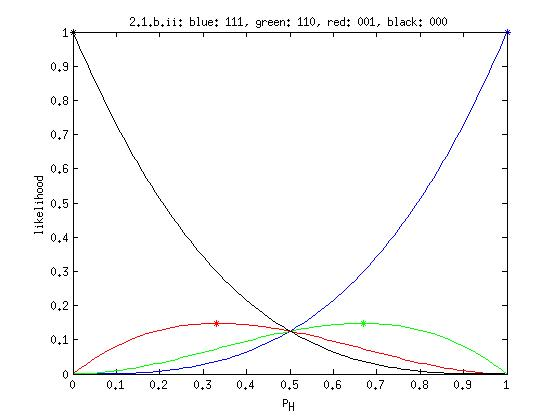
\includegraphics[scale=0.75]{hw2_ques2_1_b_ii}\\
			\end{figure}
			\vspace{0.0001em}\\
			These estimates do make sense given the data. It is obvious that the $p_H$ that maximizes the likelihood of getting 3 heads in a row (sequence [111]) is when $p_H$ = 1. The intuition is the same for getting all tails (sequence [000]). The likelihood of getting sequence [110] out of 3 coin flips is maximized when the probability of getting heads is 2/3. Similarly, the maximum likelihood of flipping 2 tails out of 3 coin flips is when the probability of getting heads is equal to 1 out of 3 flips.
			\vspace{0.5em}\\
			\item
			$\text{[000]: }\int\limits_0^1p_H^0(1-p_H)^3dp_H=\int\limits_0^1(1-p_H)^3dp_H=\left.(-1)\frac{1}{4}(1-p_H)^4\right|_0^1=\frac{-1}{4}\big((1-1)^4-(1-0)^4\big)=\frac{1}{4}$\\
			$\text{[111]: }\int\limits_0^1p_H^3(1-p_H)^0dp_H=\int\limits_0^1p_H^3dp_H=\left.\frac{1}{4}p_H^4\right|_0^1=\frac{1}{4}(1^4-0^4)=\frac{1}{4}$\\
			$\text{[110]: }\int\limits_0^1p_H^2(1-p_H)^1dp_H=\int\limits_0^1(p_H^2-p_H^3)dp_H=\left.(\frac{1}{3}p_H^3-\frac{1}{4}p_H^4)\right|_0^1=\frac{1}{3}-\frac{1}{4}=\frac{1}{12}$\\
			$\text{[001]: }\int\limits_0^1p_H^1(1-p_H)^2dp_H=\int\limits_0^1p_H(1-p_H^2)dp_H=\int\limits_0^1p_H(1-2p_H+p_H^2)dp_H\\=\int\limits_0^1(p_H-2p_H^2+p_H^3)dp_H=\left.(\frac{1}{2}p_H^2-\frac{2}{3}p_H^3+\frac{1}{4}p_H^4)\right|_0^1=\frac{1}{2}-\frac{2}{3}+\frac{1}{4}=\frac{1}{12}$\vspace{0.5em}\\
			You can tell that this is not a valid probability distribution over $p_H$ because the total sum of the area under these curves is not equal to 1. The reason that it's invalid is because these 4 sequences are only a subset of the total possible sequences, (for example, we are missing [101], [100], etc.). 
		\end{enumerate}
		\item We choose $p_H$ that maximizes the probability of the observed sequence. We find this value of $p_H$ by maximizing the likelihood function.
		\vspace{0.5em}\\
		$\hat{p}_H=\underset{p_H}{\mathrm{\text{arg max}}}P(H_1,\text{...},H_{N_{bits}};p_H)=\underset{p_H}{\mathrm{\text{arg max}}}\big(p_H^{N_H}(1-p_H)^{N_{bits}-N_H}\big)$
		\vspace{0.5em}\\
		There are different techniques that can be used to find the value of $p_H$ that maximizes the likelihood function (e.g. taking the derivative, gradient descent). To find this maximizing value, we can take the derivative of this likelihood function, set it equal to 0, and solve for $p_H$ since a closed-form solution exists for this particular likelihood function.
		\vspace{0.5em}\\
		Instead of maximizing the likelihood function, we will instead maximize the log-likelihood function which reaches its maximum value at the same points as the original function, (this is because the logaritm function is monotonically increasing).
		\vspace{0.5em}\\
		$\hat{p}_H=\underset{p_H}{\mathrm{\text{arg max  }}}log\big(P(H_1,\text{...},H_{N_{bits}};p_H)\big)=\underset{p_H}{\mathrm{\text{arg max  }}}log\big(\big(p_H^{N_H}(1-p_H)^{N_{bits}-N_H}\big)\big)\\=\underset{p_H}{\mathrm{\text{arg max  }}}log(p_H^{N_H})+log(1-p_H)^{N_{bits}-N_H}=\underset{p_H}{\mathrm{\text{arg max  }}}N_Hlog(p_H)+(N_{bits}-N_H)log(1-p_H)$
		\vspace{1.0em}\\
		Now take the derivative of the log-likelihood function:
		\vspace{1.0em}\\
		$\frac{d}{dp_H}\big(N_Hlog(p_H)+(N_{bits}-N_H)log(1-p_H)\big)=\frac{N_H}{p_H}-\frac{N_{bits}-N_H}{1-p_H}$
		\vspace{1.0em}\\
		Set it equal to 0 and solve for $p_H$:
		\vspace{1.0em}\\
		$\frac{N_H}{p_H}-\frac{N_{bits}-N_H}{1-p_H}=0$\\
		\vspace{0.5em}\\
		$\frac{N_H}{p_H}=\frac{N_{bits}-N_H}{1-p_H}$\\
		\vspace{0.5em}\\
		$\frac{N_H(1-p_H)}{p_H}=N_{bits}-N_H$\\
		\vspace{0.5em}\\
		$\frac{1-p_H}{p_H}=\frac{N_{bits}-N_H}{N_H}$\\
		\vspace{0.5em}\\
		$\frac{1}{p_H}-1=\frac{N_{bits}}{N_H}-1$\\
		\vspace{0.5em}\\
		$p_H=\frac{N_H}{N_{bits}}$
		\vspace{1.0em}\\
		This result shows that the maximizing value of $p_H$ is the number of heads (or 1-bits) divided by the total number of coin tosses (or bits).
	\end{enumerate}
	\item
		\begin{enumerate}
		\item
               	$L(O_1,{...},O_{N_{bits}};p_H)=P(O_1,{...},O_{N_{bits}};p_H)=\prod_{i=1}^{N_{bits}}P(O_i;p_H)$\\
		\vspace{0.001em}\\
		$=\prod_{i=1}^{N_{bits}}\sum_{t=0}^1P(O_i,H_i=t;p_H)=\prod_{i=1}^{N_{bits}}\sum_{t=0}^1P(O_i|H_i=t;p_H)P(H_i=t;p_H)$\\
		\vspace{0.001em}\\
		$=\prod_{i=1}^{N_{bits}}P(O_i|H_i=0;p_H)P(H_i=0;p_H)+P(O_i|H_i=1;p_H)P(H_i=1;p_H)$\\
		\vspace{0.001em}\\
		$=\prod_{i=1}^{N_{bits}}P(O_i|H_i=0;p_H)(1-p_H)+P(O_i|H_i=1;p_H)p_H\\$
		\vspace{0.01em}\\
		Given: $O_i=H_i+\epsilon_i\text{, }\epsilon{i}\sim{}N(0,\sigma^2)$\\
		\vspace{0.001em}\\
		$H_i=t:\hspace{1em}O_i=t+\epsilon_i$\hspace{2em}Solve for $\epsilon_i:$\hspace{2em}$\epsilon_i=O_i-t$\\
		\vspace{0.001em}\\
		$t=0:$\hspace{2em}$N(O_i;0,\sigma^2)$\hspace{2em}$t=1:$\hspace{2em}$N(O_i-1;0,\sigma^2)$\\
		\vspace{0.01em}\\
		$L(O_1,{...},O_{N_{bits}};p_H)=\prod_{i=1}^{N_{bits}}=N(O_i;0,\sigma^2)(1-p_H)+N(O_i-1;0,\sigma^2)p_H$\\
		\vspace{0.01em}\\
		Let $\alpha_i=N(O_i;0,\sigma^2)$ and $\beta_i=N(O_i-1;0,\sigma^2)$\\
		\vspace{0.01em}\\
		$L(O_1,{...},O_{N_{bits}};p_H)=\prod_{i=1}^{N_{bits}}\alpha_i(1-p_H)+\beta_ip_H$\\
		\vspace{0.001em}\\
		\Large$L(O_1,{...},O_{N_{bits}};p_H)=\prod_{i=1}^{N_{bits}}p_H(\beta_i-\alpha_i)+\alpha_i$\\
		\vspace{0.001em}\\
		\Large$LL(O_1,{...},O_{N_{bits}};p_H)=\sum_{i=1}^{N_{bits}}log(p_H(\beta_i-\alpha_i)+\alpha_i)$\\
		\vspace{0.001em}\\
		\normalsize\text{Check concavity: check 2nd derivative}\\
		\vspace{0.001em}\\
		$\frac{dLL}{dp_H}=\sum_{i=1}^{N_{bits}}\frac{\beta_i-\alpha_i}{p_H(\beta_i-\alpha_i)+\alpha_i}$\\
		\vspace{0.001em}\\
		$\frac{d^2LL}{dp_H^2}=\sum_{i=1}^{N_{bits}}-\big(\frac{\beta_i-\alpha_i}{p_H(\beta_i-\alpha_i)+\alpha_i}\big)^2$\\
		\vspace{0.001em}\\
		The expression inside the parenthesis is always squared so it's guaranteed to be positive. The whole expression is then multiplied by -1 and we take the summation of all of these expressions. This shows that the second derivative is \textit{always} negative for all values of $p_H$. \\
		\vspace{0.001em}\\
		Concavity is important because it means there exists a value of some variable that minimizes/maximizes the function we are optimizing. These mins and maxs can be local or (hopefully) global.\\
		\vspace{0.001em}\\
		\item
		$\hat{p}_H=\underset{p_H}{\mathrm{\text{arg max}}}\sum_{i=1}^{N_{bits}}log(p_H(\beta_i-\alpha_i)+\alpha_i)$\\
		\vspace{0.001em}\\
		There is no closed-form solution to this equation. We can use iterative convergence methods, like gradient descent, to obtain the MLE. \\
		\item  Log-likelihood vs $p_H$\\
		\vspace{0.001em}\\
		\begin{figure}[h]
		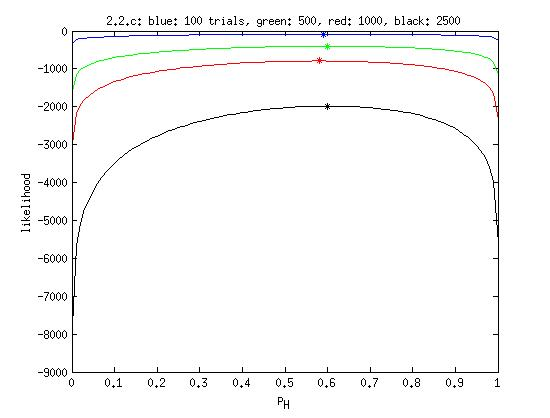
\includegraphics[scale=0.75]{hw2_ques2_2_c}
		\end{figure}
		When we increase $\sigma^2$, the noise deviates more from the mean which means we get more bit errors. This causes the curves on the graph to flatten out since other $p_H$s become more likely and the likelihood of $\hat{p}_H$ decreases.
		\vspace{0.001em}\\
		\item $\hat{p}_H$, $\bar{p}_H$ vs Trial Size (see graph 2.2.d)\\
		
		\begin{figure}[h]
		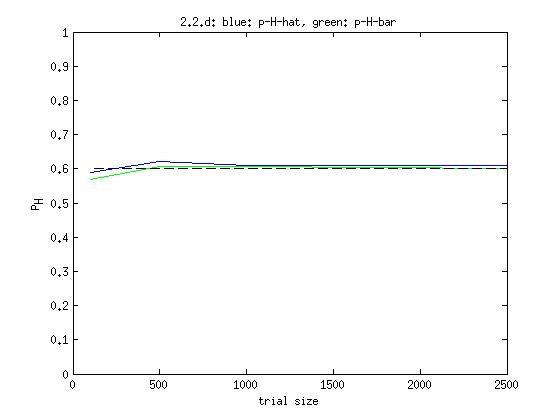
\includegraphics[scale=0.75]{hw2_ques2_2_d}
		\end{figure}
		$\bar{p}_H$  is the ratio of the observed number of 1-bits to the total number of bits. As $\sigma^2$ approaches 0, $\hat{p}_H$ is approximately equal to $\bar{p}_H$ because the noise does not deviate far from 0 (the mean) so the bits are unlikely to be corrupted. When the variance is 0.1, $\bar{p}_H$ and $\hat{p}_h$ still perform similarly, however, $\hat{p}_H$ performs slightly better for trial sizes greater than 500 (this can be seen on graph 2.2.d). As we increase $\sigma^2$ further, the accuracy of $\hat{p}_H$ compared with $\bar{p}_H$ increases as well \textit{as long as the trial size is sufficiently large}.
		\vspace{0.001em}\\
		\end{enumerate}
		\item
		\begin{enumerate}
		\item $LL(O_1,{...},O_{N_{bits}};p_H)=\sum_{i=1}^{N_{bits}}log(p_H(\beta_i-\alpha_i)+\alpha_i)$\\
		\vspace{0.001em}\\
		Where: \hspace{2em}$\alpha_i\sim{}N(O_i;0,\sigma_i^2)$\hspace{2em}$\beta_i\sim{}N(O_i-1;0,\sigma_i^2)$\\
		\vspace{0.001em}\\
		Changing the model to include a sigma that grows with consecutive bits is independent of $p_H$ and does not change the first or second derivative with respect to $p_H$ (see part 2a). Therefore, the log-likelihood function is still concave.
		\item Log-likelihood vs $p_H$ (see graph 2.3.b)
		\begin{figure}[h]
		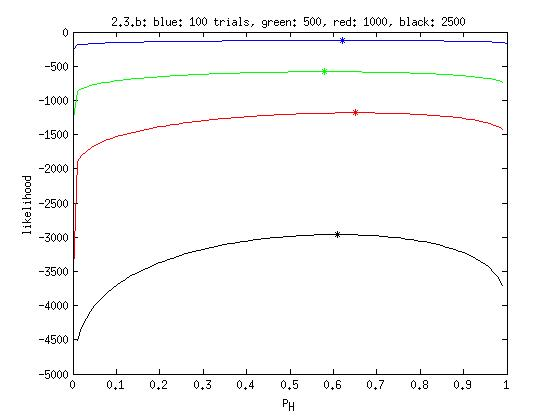
\includegraphics[scale=0.75]{hw2_ques2_3_b}
		\end{figure}
		\item $\hat{p}_H$, $\bar{p}_H$ vs Trial Size (see graph 2.3.c)\\
		$\bar{p}_H$ does better until the trial size is at least 500. After this point, $\hat{p}_H$ performs better but also starts moving away from $p_H^*$ as the trial size increases past around 1500.
		\begin{figure}[h]
		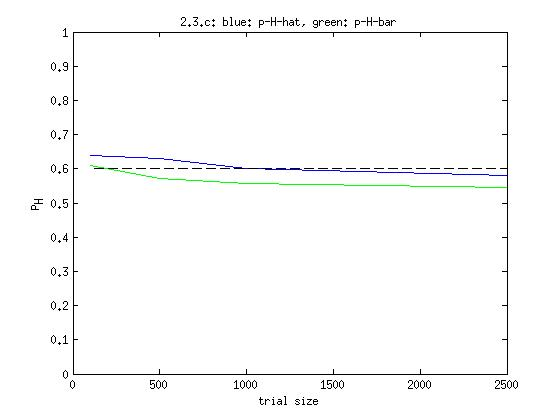
\includegraphics[scale=0.75]{hw2_ques2_3_c}
		\end{figure}
		\end{enumerate}
\end{enumerate}

\end{document}